\chapter{Regole di Associazione}
    $\textbf{Association Rules}$ è un metodo per l'identificazione di patterns frequenti, correlazioni, associazioni o strutture causali in set di dati.
    \\[1\baselineskip]
    Dato un insieme di transazioni, l'obiettivo dell'Association Rule Mining è trovare le regole che ci consentono di prevedere l'occorrenza di un elemento specifico in base alle occorrenze degli altri elementi nella transazione.
    \\[1\baselineskip]
    Una regola di associazione è normalmente rappresentata nella forma $\{X\} \Rightarrow \{Y\}$ dove:
        \begin{itemize}
            \item $\{X\}$ è la parte $\textit{antecedente}$ (if), ovvero qualcosa che si trova nei dati;
            \item $\{Y\}$ è la parte $\textit{conseguente}$ (then), ovvero qualcosa che si trova in congiunzione con la parte antecedente.
        \end{itemize}

    Un esempio è la seguente frase: "Se un cliente acquista il pane, ha il 70\% di probabilità di acquistare il latte".
    \\
    Il pane è l'antecedente nella regola associativa, mentre il latte è il conseguente.

    \clearpage

    \section{Definizioni}
        Utilizziamo questa tabella per capire meglio le varie definizioni che verranno a breve illustrate:
        
        \begin{figure}[h]
            \centering
            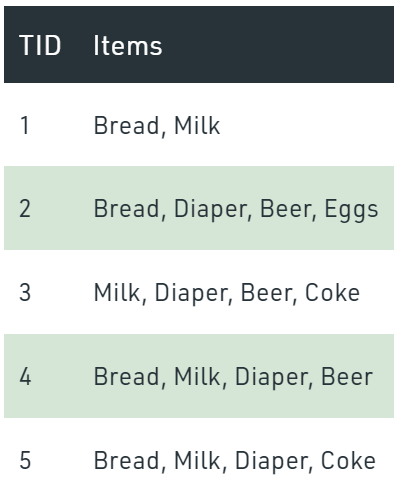
\includegraphics[width = 5cm, height = 4cm]{tabella-supporto-regole-associative.png}
        \end{figure}

        \begin{itemize}
            \item $\textbf{Supporto}:$ annotato come $S \left( X \right)$, è la frequenza di apparizione di $X$ nella tabella.
                Se applicato a una regola, $S \left( X \Rightarrow Y \right)$ è la frequenza di apparizione di $X \cup Y$ e ci indica quante volte appare la regola $X \Rightarrow Y$ nella tabella.
                \\[1\baselineskip]
                Per esempio, $S \left( \textrm{\{Milk, Bread\}} \Rightarrow \textrm{\{Diaper\}} \right) =$
                \\[0.2\baselineskip]
                $\frac{\#(\textrm{\{Milk, Bread\}} \cup \{Diaper\})}{\#\textrm{transazioni}} = \frac{2}{5} = 40\%$.
                \\[0.5\baselineskip]

            \item $\textbf{Confidenza}:$ annotata come $C \left( X \Rightarrow Y \right)$, indica il rapporto tra il numero di volte che appare $Y$ nelle transazioni che includono anche $X$ e il numero di volte che appare $X$.
                \\[1\baselineskip]
                Per esempio, $C \left( \textrm{\{Bread\}} \Rightarrow \textrm{\{Beer\}} \right) = \frac{2}{4} = 50\%$
        \end{itemize}

    \section{Algoritmi}
        \begin{itemize}
            \item $\textbf{Apriori}:$ È utilizzato per la generazione degli itemset frequenti, per approssimazioni successive, a partire dagli itemset con un solo elemento.
                \\[1\baselineskip]
                In sintesi, il presupposto teorico su cui si basa l'algoritmo parte dalla considerazione che se un insieme di oggetti (itemset) è frequente, allora anche tutti i suoi sottoinsiemi sono frequenti, ma se un itemset non è frequente, allora neanche gli insiemi che lo contengono sono frequenti.

            \item $\textbf{FP-Growth}:$ (FP = Frequent Pattern) È un modo alternativo per trovare set di items frequenti senza utilizzare la generazione di candidati, migliorando così le prestazioni.
                \\[1\baselineskip]
                Usa una strategia $\textit{divide et impera}$: il fulcro di questo metodo è l'utilizzo di una speciale struttura di dati denominata Frequent-Pattern Tree (FP-tree), che conserva le informazioni sull'associazione del set di elementi.
                \\[1\baselineskip]
                Usando questa strategia, FP-Growth riduce i costi di ricerca cercando ricorsivamente pattern brevi e poi concatenandoli in dei pattern frequenti più lunghi.
        \end{itemize}

        \begin{figure}[h]
            \caption{Esempio di Apriori}
            \centering
            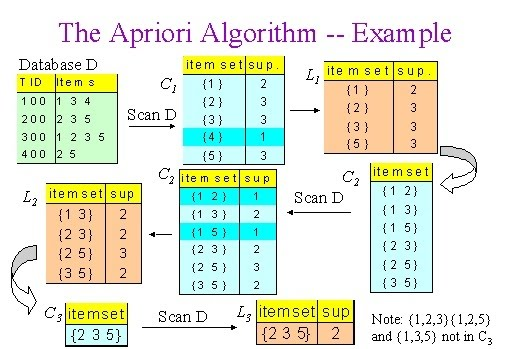
\includegraphics[width = 10cm]{apriori-example.jpg}
        \end{figure}

        \begin{figure}[h]
            \caption{Esempio di FP-Growth}
            \centering
            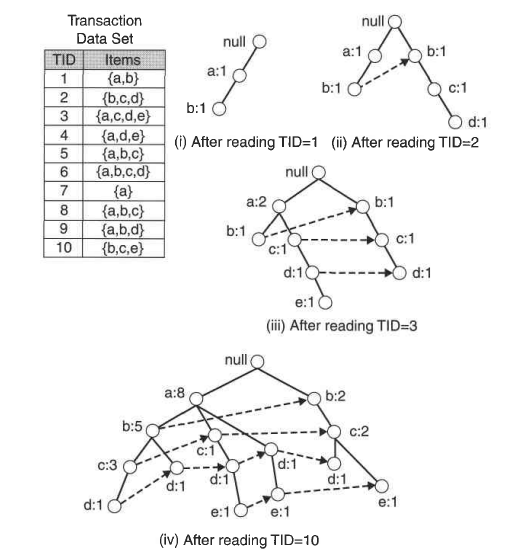
\includegraphics[width = 10cm]{FP-tree-example.png}
        \end{figure}

\clearpage